%!TEX root = ../report.tex

\begin{document}
    \chapter{Introduction}

The development of Deep Neural Networks (DNNs) made tasks such as object classification \cite{alexnet} and object detection \cite{fasterrcnn}, \cite{fastrcnn} easy to solve.
These DNNs has been deployed in various real world scenarios such as autonomous driving \cite{autonomousdriving}, semi-autonomous robotic surgery \cite{roboticsurgery} and also in space rovers \cite{Marsrover_1}, \cite{Marsrover_2}.
DNNs are majorly deployed in the perception stack in the autonomous driving pipeline. 
Figure~\ref{fig:Apollopipeline} depicts the pipeline of the modules present in one of the open source autonomous driving platform called Apollo \cite{baiduapollo}.
From this pipeline, one can infer that the most of the decisions in the prediction and motion planning module of the autonomous car is dependent on the output of the perception module.
Since the perception module plays such significance, the developers of the perception stack must make sure the outputs are meaningful.
\begin{figure}[h!]
    \centering
    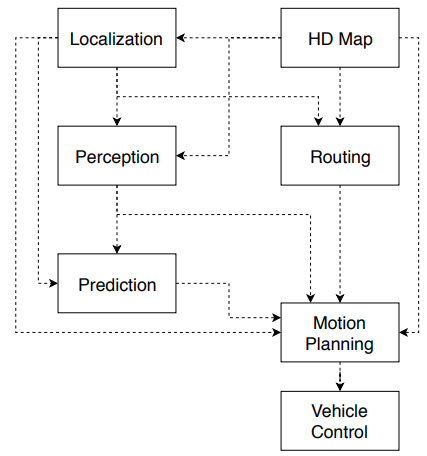
\includegraphics[scale=0.35]{images/Apollopipeline.png}
    \caption{Module pipeline for Apollo autonomous driving platform. Image taken from \cite{baiduapollo}}
    \label{fig:Apollopipeline}
\end{figure}

The DNNs utilized in perception module need to be trained on the dataset which should be similar to area of its deployment.
For example, an autonomous driving agent must be trained on dataset containing roads, vehicles, vegetation and other objects found around road.
This closedness of the dataset i.e., fixed number of classes, will cause an issue when the DNN encounter an unknown object in real world.
This unknown object is predicted as one of the class in the dataset, leading to radical decisions when this error is propogated down the pipeline in Figure \ref{fig:Apollopipeline}.
One such real world problem is encountered by the Tesla autonomous driving platform.
\begin{figure}[h!]
    \begin{subfigure}{0.48\textwidth}
        \centering
        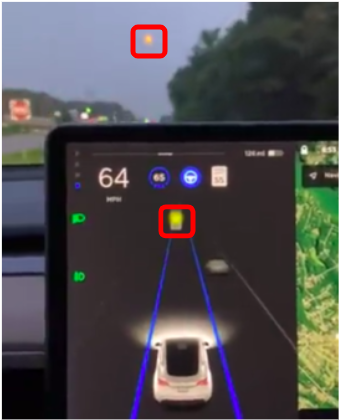
\includegraphics[scale=0.5]{images/tesla_1.png}
        \caption{}
        \label{fig:teslafails_1}
    \end{subfigure}
    \begin{subfigure}{0.48\textwidth}
        \centering
        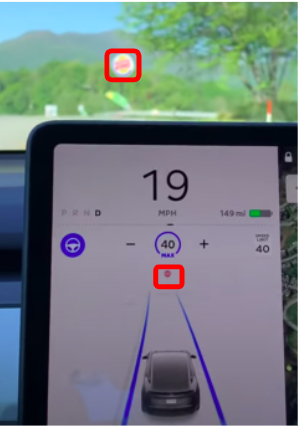
\includegraphics[scale=0.5]{images/tesla_2.png}
        \caption{}
        \label{fig:teslafails_2}
    \end{subfigure}
    \caption{Misdetection of OOD objects in Tesla autonomous driving platform. (a) Moon is detected as yellow signal light and (b) depicts the misdetection of burger king sign as stop traffic sign. Images taken from \cite{tesla_fails}}
\end{figure}

Figure~\ref{fig:teslafails_1} and Figure~\ref{fig:teslafails_2} depicts the misdetections from the Tesla autonomous driving system.
The problem in the first image, is the moon is detected as the yellow signal light and second image has the problem of misdetection of burger king sign as stop signal.
These misdetections of unknown objects in the environment might lead to fatal consequences.
This questions the safety of the Deep Neural Networks (DNNs) predictions and so an effort has been made in this thesis to detect these unknown objects in 3D LiDAR data using uncertainty score.
The unknown obejcts in the real world which are not present in the training dataset can be regarded as out-of-distribution (OOD) objects. 
More discussion on the OOD is presented in Section~\ref{sec:oodvanom}.

\section{OOD/Anomaly/Distributional shift}
\label{sec:oodvanom}
\begin{figure}[h!]
    \begin{subfigure}{0.333\textwidth}
        \centering
        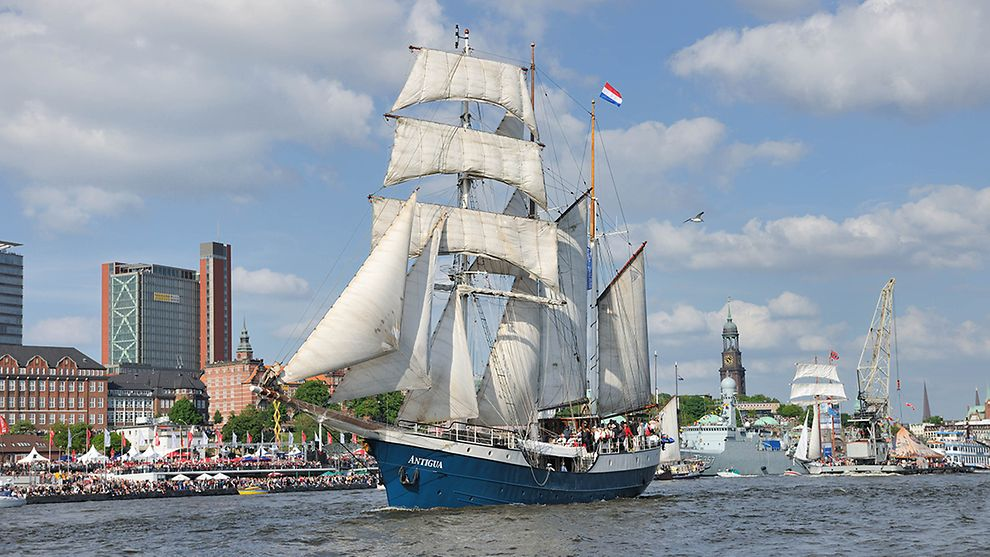
\includegraphics[height=0.15\textheight,width=0.95\textwidth]{images/intro_ood_anomaly/old_ship.jpg}
        \caption{}
        \label{fig:old_ship}
    \end{subfigure}
    \begin{subfigure}{0.333\textwidth}
        \centering
        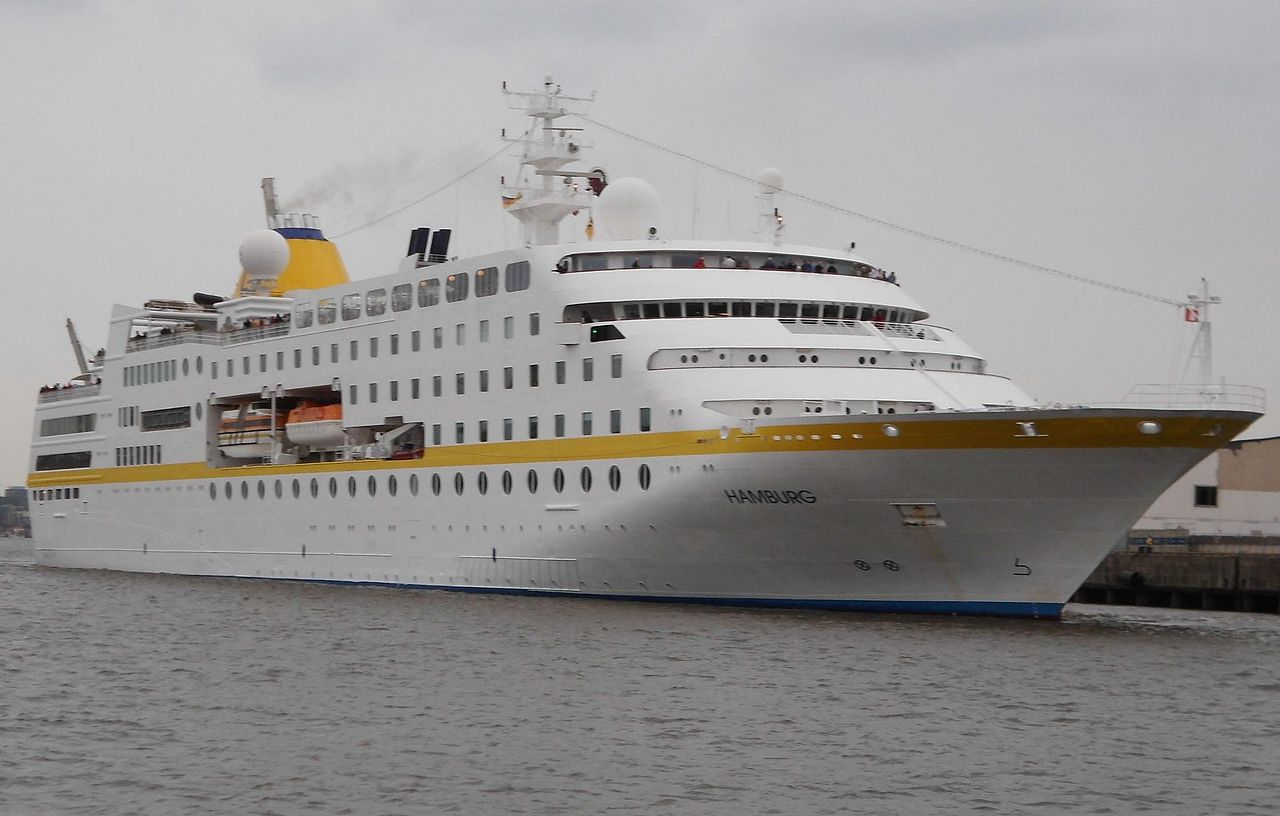
\includegraphics[height=0.15\textheight,width=0.95\textwidth]{images/intro_ood_anomaly/Trainer_cruiser.jpeg}
        \caption{}
        \label{fig:trian_cruiser}
    \end{subfigure}
%\end{figure}
%\begin{figure}[h!]
    \begin{subfigure}{0.333\textwidth}
        \centering
        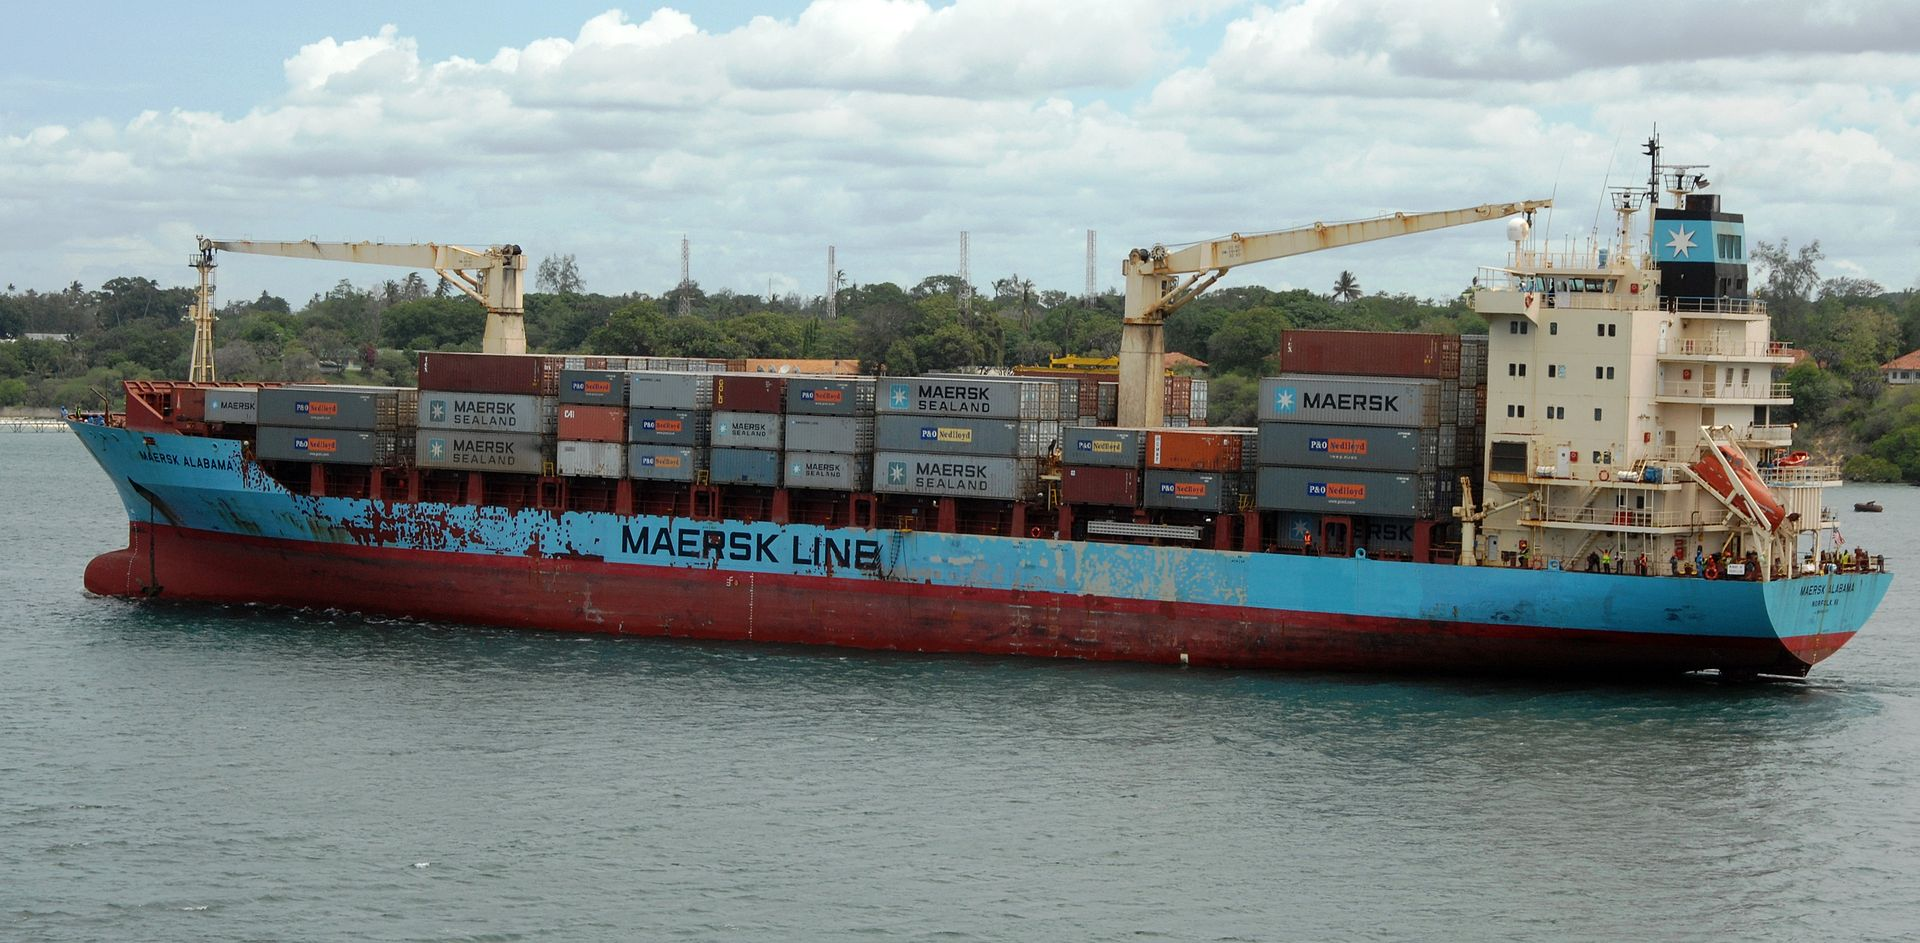
\includegraphics[height=0.15\textheight,width=0.95\textwidth]{images/intro_ood_anomaly/Anomaly_container.jpg}
        \caption{}
        \label{fig:anom_container}
    \end{subfigure}
    \begin{subfigure}{0.333\textwidth}
        \centering
        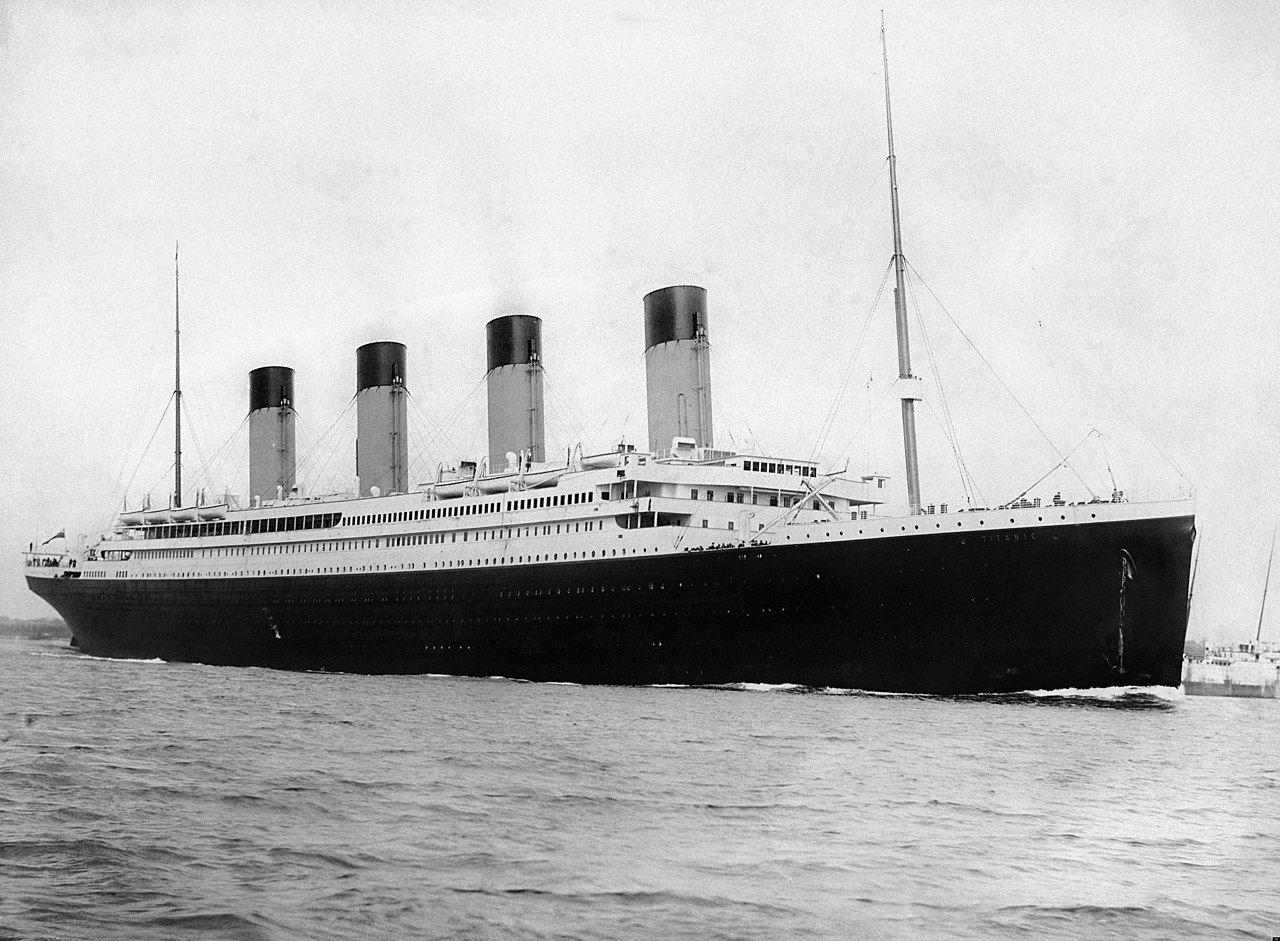
\includegraphics[height=0.15\textheight,width=0.95\textwidth]{images/intro_ood_anomaly/Anomaly_titanic.jpg}
        \caption{}
        \label{fig:anom_titanic}
    \end{subfigure}
    \begin{subfigure}{0.333\textwidth}
        \centering
        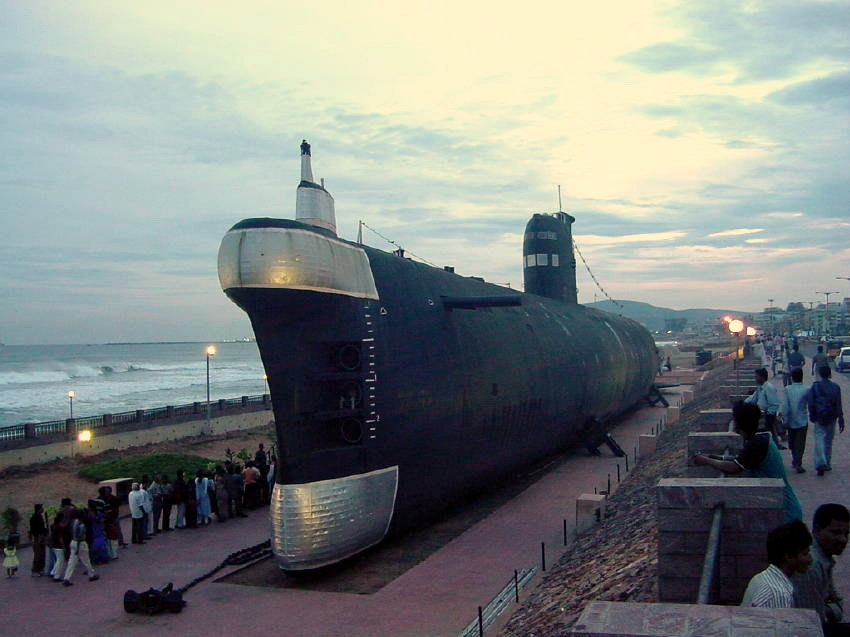
\includegraphics[height=0.15\textheight,width=0.95\textwidth]{images/intro_ood_anomaly/ood_submarine.jpg}
        \caption{}
        \label{fig:ood_submarine}
    \end{subfigure}
    \begin{subfigure}{0.333\textwidth}
        \centering
        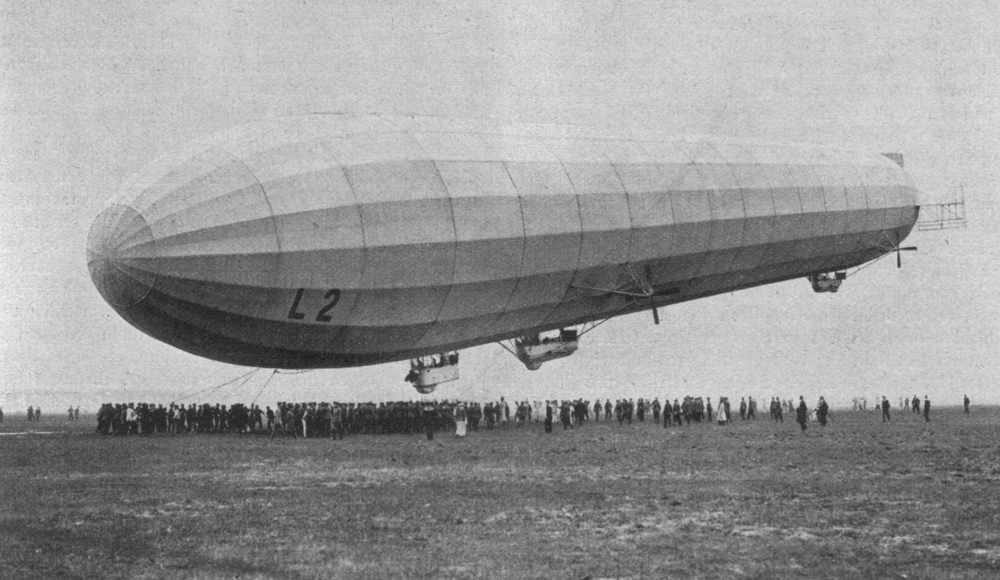
\includegraphics[height=0.15\textheight,width=0.95\textwidth]{images/intro_ood_anomaly/ood_airship.jpg}
        \caption{}
        \label{fig:ood_airship}
    \end{subfigure}
    \caption{Illustration of distributional shift, anomaly and out of distribution examples using various kind of ships. (a) represents the sail ship during 18th century. (b) depicts the current training data.
    (c), and (d) represents the anamolous ship data and (e), and (f) represents the OOD data. Images are taken from \cite{old_ship}, \cite{train_cruiser}, \cite{container},
    \cite{titanic}, \cite{submarine}, and \cite{airship} respectively in the order they appear.}
\end{figure}

Let us time travel back to $18^{th}$ century and assume that we had implemented a DNN model to detect ships, the dataset images for training the DNN model will be similar to Figure~\ref{fig:old_ship}.
$18^{th}$ century ships as in Figure~\ref{fig:old_ship} can be defined as ``\textit{ship contains hull and sails}''.
Fast forward to present time, current ships are as shown in Figure \ref{fig:trian_cruiser}.
Ship as in \ref{fig:trian_cruiser} can be defined as ``\textit{ship contains hull and passenger decks stacked upon each other}''.
Now if we want to deploy the old model trained with old ships to detect the present generation of ships, it is diffcult because of the change in definition and properties of ship. 
This change in data distribution over a period of time is called ``\textit{distributional shift}'' of the data.

Anomaly can be defined as the patterns that doesn't conform to the expected training behavior as proposed in \cite{anomaly_sec1_1}.
By this definition, Figure \ref{fig:anom_container} and Figure \ref{fig:anom_titanic} can be considerd as anomalies.
This is becuase Figure \ref{fig:anom_container} is a container ship looking similar to Figure \ref{fig:trian_cruiser} instead of passenger decks we have containers stacked.
Figure \ref{fig:anom_titanic} is also anomaly because the Titanic also has a hull, passenger decks and chimneys. 
This additional chimnies as a fetures deviates this image from the definition of the ship and can be considered as ``\textit{anomaly}''.

The input for out of distribution (OOD) is drawn from an unknown distribution of unknown data, which is not near to the trianing distribution.
Figure~\ref{fig:ood_submarine} and Figure~\ref{fig:ood_airship} are submarine and airship doesn't adhere to the definition of ship by any means.
In general, one can argue that OOD can be defined as inputs which doesn't belong to any class in the training data.
This kind of problem can also be called as Open Set Recognition (OSR) problem.


%\begin{figure}[h!]
%    \begin{subfigure}{0.333\textwidth}
%        \centering
%        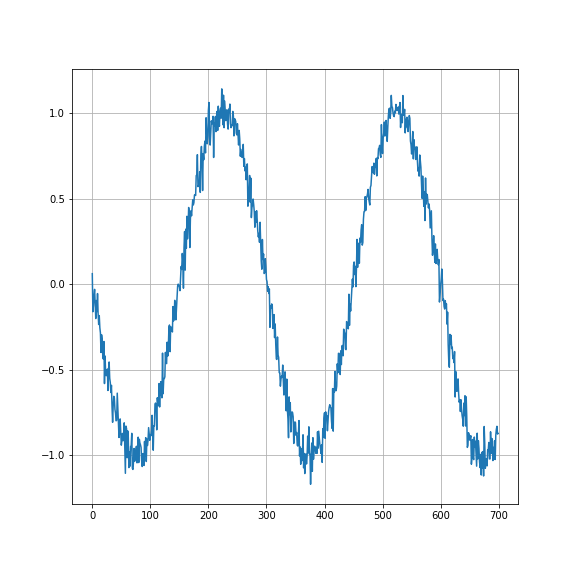
\includegraphics[height=0.3\textheight,width=0.98\textwidth]{images/intro_ood_anomaly/normal_train.png}
%        \caption{}
%        \label{fig:normal_train_time}
%    \end{subfigure}
%    \begin{subfigure}{0.333\textwidth}
%        \centering
%        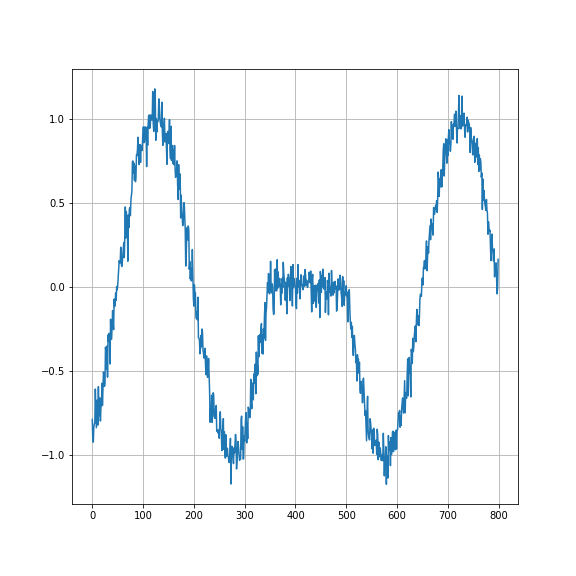
\includegraphics[height=0.3\textheight,width=0.98\textwidth]{images/intro_ood_anomaly/anomaly_train.png}
%        \caption{}
%        \label{fig:anomaly_time}
%    \end{subfigure}
%    \begin{subfigure}{0.333\textwidth}
%        \centering
%        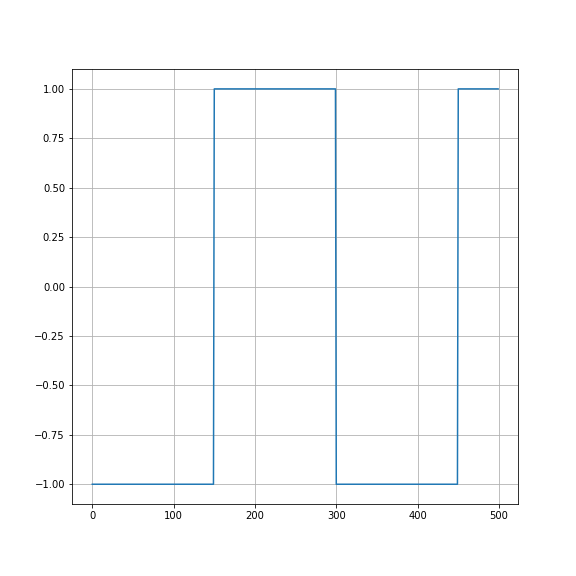
\includegraphics[height=0.3\textheight,width=0.98\textwidth]{images/intro_ood_anomaly/ood_train.png}
%        \caption{}
%        \label{fig:ood_time}
%    \end{subfigure}
%    \caption{Illustration of anomaly and OOD with time series data as example. \ref{fig:normal_train_time} depicts the triaining data as sinusoidal wave.
%    \ref{fig:anomaly_time} represents the anomaly in the sinusoidal wave and \ref{fig:ood_time} represents the square wave as OOD signal}
%\end{figure}

\section{Problem Statement}
In this thesis, we study the application of out-of-distribution (OOD) detection over the 3D semantic segmentation problem in the context of autonomous driving.
Notably, we study the 3D semantic segmentation datasets available and create a benchmark for in-distribution and out-distribution for the OOD setting.

The other major issue, we address in this thesis is the OOD detection methods themselves.
Existing OOD detection methods are developed on 2D classification and 2D semantic segmentation tasks and applicability of these methods on 3D semantic segmentation tasks is not studied. 
This is also challenging because the existing OOD methods are not easily adaptable to the 3D segmentation models because segmentation involves multi class classification and moreover high dimensionality of the 3D data impose computational constraints.
\newline

The research questions answered by this thesis are:
\begin{itemize}
    \item[\textbf{R1}] How to create a benchmark over 3D segmentation datasets for the OOD setting?, i.e., create the in-distribution and out-distribution datasets.
    \item[\textbf{R2}] How to extend current OOD detection methods from 2D classification task to 3D semantic segmentation?
    \item[\textbf{R3}] Is uncertainty quantification an effective approach to classify OOD detection in 3D semantic segmentation models?
    % \item[\textbf{R4}] What metrics can be applied for the OOD detection task over 3D semantic segmentation models? 
    \item[\textbf{R4}] How to evaluate the OOD detections over the 3D semantic segmentation task?
\end{itemize}

\subsection{Contributions}
The contributions made in this thesis are
\begin{enumerate}
    \item A complete survey on the available 3D LiDAR datasets
    \item A detailed survey on existing 3D semantic segmentation models
    \item Benchmarking of 3D LiDAR datasets for OOD detection. Proposed two benchmark datasets Sematic3D vs S3DIS and Semantic3D vs Semantic3D without color with Semantic3D being training dataset and S3DIS and Semantic3D without color being OOD datasets.
    \item A survey on the uncertainty estimation methods and classical OOD methods.
    \item An evaluation of OOD on benchmarked datasets over RandLA-Net model using Deep ensemble technique for uncertainty estimation.
\end{enumerate}

To summarize this chapter, we discussed the motivation behind the problem of OOD detection like how errors in perception results lead to catastrophic consequences in an autonomous driving pipeline.
Also discussed in detail about what an OOD and Anomaly are using a ship example and finally we discussed the contributions of this thesis.
The following chapters include study of the state of the art, experimentation details and then followed by results and conclusion chapters.
\end{document}
